\documentclass[12pt, amssymb, one column]{article}
\usepackage{times, amsthm, amsmath, amssymb, cancel, changepage, graphicx, lipsum, fancyhdr, mathabx, enumitem}
\usepackage[margin=1in]{geometry}

\newcommand{\ihat}{\mathbf {\hat \imath}}
\newcommand{\jhat}{\mathbf {\hat \jmath}}

\pagestyle{fancy}
\fancyhf{}
\rhead{Due: October 10, 2019}
\chead{\bf{Homework 5}}
\lhead{BIOST 2081}
\cfoot{-\thepage-}

\setitemize[0]{leftmargin=.3in}
\renewcommand{\baselinestretch}{.9}


%end of header, beginning of document

\begin{document}

\begin{itemize}
	\item[1.] Compute $\iint_R 2xy-x^2+1 \mathop{dA} $ over $R=[2,3] \times [-1,1]$ in the order given below.
	\begin{itemize}
		\item[(a)] Integrate with respect to $x$ first then $y$.
		\item[(b)] Integrate with respect to $y$ first then $x$.
	\end{itemize}
	
	\item[2.] Integrate each of the following:
		\begin{itemize}
			\item[(a)] $\iint_R y^5-x^2e^y \mathop{dA}, \,\, R=[-1,2] \times [0,4]$
			\item[(b)] $\iint_R \frac{\ln(4xy)}{xy} \mathop{dA}, \,\, R=[1,2]\times[3,4]$
			\item[(c)] $\iint_D 12x^2y-y^2 \mathop{dA}, \,\, D=\{(x,y)|-2\leq x \leq 2, -x^2 \leq y \leq x^2\}$
			\item[(d)] $\iint_D 7y^3e^{x^2+1} \mathop{dA}$ where $D$ is the region bounded by $y=2\sqrt[4]{x},x=9$ and the x-axis
			\item[(e)] $\iint_D 9-\frac{6y^2}{x^2} \mathop{dA}$ where $D$ is the region in the first quadrant bounded by $y=x^3$ and $y=4x$.
		\end{itemize}
	
	\item[3.] Integrate the following functions over their corresponding regions
	\begin{figure}[h]
		\centering
		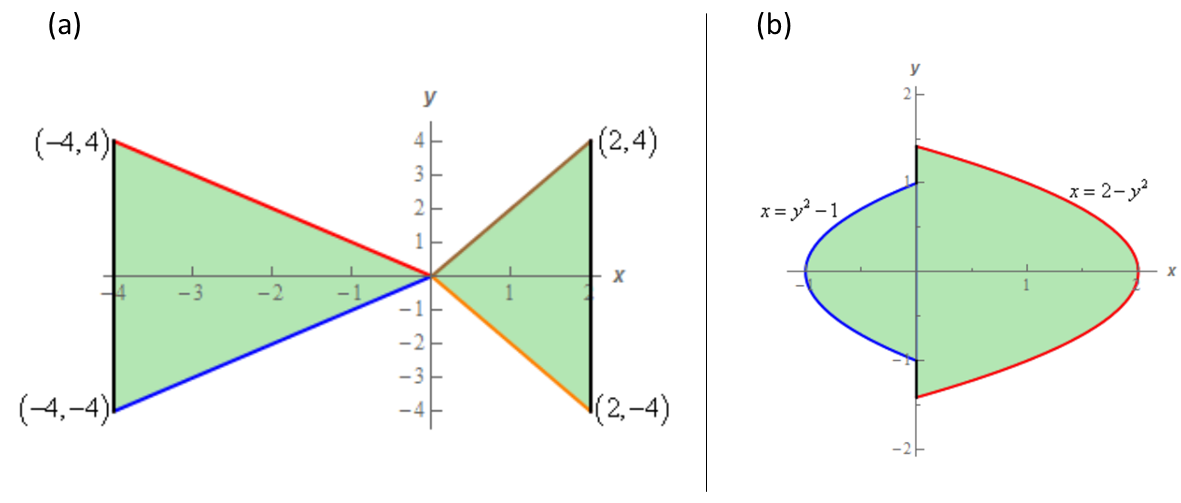
\includegraphics[width=.8\textwidth]{regions.png}\\
	\end{figure}
		\begin{itemize}
			\item[(a)] $f(x,y) = xy-y^2$
			\item[(b)] $f(x,y) = 6y^2 + 10yx^4$
		\end{itemize}
	
	\item[4.] Evaluate $\iint_D xy-y^3 \mathop{dA}$ where $D$ is the region bounded by $y=x^2, y=-x^2,$ and $x=2$ in the order given below
		\begin{itemize}
			\item[(a)] Integrate with respect to $x$ first then $y$.
			\item[(b)] Integrate with respect to $y$ first then $x$.
		\end{itemize}
	
	\item[5.] Determine the region we would get by applying the given transformation $T$ to region $R$ for each below.
		\begin{itemize}
			\item[(a)] $R$: region inside $\frac{x^2}{25}-49y^2=1$, $T: x=5u, y=\frac{1}{7}v$
			\item[(b)] $R$: region bounded by $xy=4, xy=10, y=x, y=6x$, $T: x=2\sqrt{\frac{u}{v}}, y=4\sqrt{uv}$
		\end{itemize}
	
	\item[6.] Evaluate the following integrals using the given transformation.
		\begin{itemize}
			\item[(a)] $\iint_R \frac{15y}{x} \mathop{dA}$ where $R$ is the region bounded by $xy=2, xy=6, y=4, y=10$ using the transformation $x=v, y=\frac{2u}{3v}$
			\item[(b)] $\iint_R 2y-8x \mathop{dA}$ where $R$ is the parallelogram with verticies $(6,0), (8,4), (6,8), (4,4)$ using the transformation $x=\frac{1}{4}(u-v), y=\frac{1}{2}(u+v)$
		\end{itemize}
\end{itemize}

\end{document}